% Options for packages loaded elsewhere
\PassOptionsToPackage{unicode}{hyperref}
\PassOptionsToPackage{hyphens}{url}
%
\documentclass[
]{article}
\usepackage{amsmath,amssymb}
\usepackage{lmodern}
\usepackage{ifxetex,ifluatex}
\ifnum 0\ifxetex 1\fi\ifluatex 1\fi=0 % if pdftex
  \usepackage[T1]{fontenc}
  \usepackage[utf8]{inputenc}
  \usepackage{textcomp} % provide euro and other symbols
\else % if luatex or xetex
  \usepackage{unicode-math}
  \defaultfontfeatures{Scale=MatchLowercase}
  \defaultfontfeatures[\rmfamily]{Ligatures=TeX,Scale=1}
\fi
% Use upquote if available, for straight quotes in verbatim environments
\IfFileExists{upquote.sty}{\usepackage{upquote}}{}
\IfFileExists{microtype.sty}{% use microtype if available
  \usepackage[]{microtype}
  \UseMicrotypeSet[protrusion]{basicmath} % disable protrusion for tt fonts
}{}
\makeatletter
\@ifundefined{KOMAClassName}{% if non-KOMA class
  \IfFileExists{parskip.sty}{%
    \usepackage{parskip}
  }{% else
    \setlength{\parindent}{0pt}
    \setlength{\parskip}{6pt plus 2pt minus 1pt}}
}{% if KOMA class
  \KOMAoptions{parskip=half}}
\makeatother
\usepackage{xcolor}
\IfFileExists{xurl.sty}{\usepackage{xurl}}{} % add URL line breaks if available
\IfFileExists{bookmark.sty}{\usepackage{bookmark}}{\usepackage{hyperref}}
\hypersetup{
  pdftitle={Présentation des premières données - projet-pilote de personnes-ressources},
  pdfauthor={Nicolas Bressoud},
  hidelinks,
  pdfcreator={LaTeX via pandoc}}
\urlstyle{same} % disable monospaced font for URLs
\usepackage[margin=1in]{geometry}
\usepackage{longtable,booktabs,array}
\usepackage{calc} % for calculating minipage widths
% Correct order of tables after \paragraph or \subparagraph
\usepackage{etoolbox}
\makeatletter
\patchcmd\longtable{\par}{\if@noskipsec\mbox{}\fi\par}{}{}
\makeatother
% Allow footnotes in longtable head/foot
\IfFileExists{footnotehyper.sty}{\usepackage{footnotehyper}}{\usepackage{footnote}}
\makesavenoteenv{longtable}
\usepackage{graphicx}
\makeatletter
\def\maxwidth{\ifdim\Gin@nat@width>\linewidth\linewidth\else\Gin@nat@width\fi}
\def\maxheight{\ifdim\Gin@nat@height>\textheight\textheight\else\Gin@nat@height\fi}
\makeatother
% Scale images if necessary, so that they will not overflow the page
% margins by default, and it is still possible to overwrite the defaults
% using explicit options in \includegraphics[width, height, ...]{}
\setkeys{Gin}{width=\maxwidth,height=\maxheight,keepaspectratio}
% Set default figure placement to htbp
\makeatletter
\def\fps@figure{htbp}
\makeatother
\setlength{\emergencystretch}{3em} % prevent overfull lines
\providecommand{\tightlist}{%
  \setlength{\itemsep}{0pt}\setlength{\parskip}{0pt}}
\setcounter{secnumdepth}{5}
\usepackage{multirow}
\usepackage{multicol}
\usepackage{colortbl}
\usepackage{hhline}
\usepackage{longtable}
\usepackage{array}
\usepackage{hyperref}
\ifluatex
  \usepackage{selnolig}  % disable illegal ligatures
\fi

\title{Présentation des premières données - projet-pilote de personnes-ressources}
\author{Nicolas Bressoud}
\date{janvier 2021}

\begin{document}
\maketitle

{
\setcounter{tocdepth}{2}
\tableofcontents
}
\hypertarget{etat-des-lieux-des-contacts-avec-les-classes}{%
\section{Etat des lieux des contacts avec les classes}\label{etat-des-lieux-des-contacts-avec-les-classes}}

En tout, au 23 décembre 2020, j'ai reçu officiellement les coordonnées de 6 classes :

\begin{itemize}
\tightlist
\item
  3 classes dans le cycle 1
\item
  3 classes dans le cycle 2
\end{itemize}

Après contact et demande d'autorisation de récolter des données, je me suis retrouvé dans la situation suivante :

\begin{itemize}
\tightlist
\item
  2 classes ont accepté de participer
\item
  1 classe n'a pas rendu réponse
\item
  3 classes ont refusé
\end{itemize}

Les 3 refus reposent sur les arguments de manque de temps ou de surcharge.

\hypertarget{ruxe9sumuxe9-de-luxe9chantillon}{%
\section{Résumé de l'échantillon}\label{ruxe9sumuxe9-de-luxe9chantillon}}

Le tableau \ref{tab:samp} donne une idées des 2 classes.

\begin{verbatim}
## Warning: Warning: fonts used in `flextable` are ignored because the `pdflatex`
## engine is used and not `xelatex` or `lualatex`. You can avoid this warning
## by using the `set_flextable_defaults(fonts_ignore=TRUE)` command or use a
## compatible engine by defining `latex_engine: xelatex` in the YAML header of the
## R Markdown document.
\end{verbatim}

\providecommand{\docline}[3]{\noalign{\global\setlength{\arrayrulewidth}{#1}}\arrayrulecolor[HTML]{#2}\cline{#3}}

\setlength{\tabcolsep}{8pt}

\renewcommand*{\arraystretch}{1.5}

\begin{table}

\centering

\begin{longtable}{|p{0.75in}|p{0.75in}|p{0.75in}|p{0.75in}|p{0.75in}|p{0.75in}}

\caption{Résumé de l'échantillon des 2 classes A et B}\label{tab:samp}\\

\hhline{>{\arrayrulecolor[HTML]{000000}\global\arrayrulewidth=2pt}->{\arrayrulecolor[HTML]{000000}\global\arrayrulewidth=2pt}->{\arrayrulecolor[HTML]{000000}\global\arrayrulewidth=2pt}->{\arrayrulecolor[HTML]{000000}\global\arrayrulewidth=2pt}->{\arrayrulecolor[HTML]{000000}\global\arrayrulewidth=2pt}->{\arrayrulecolor[HTML]{000000}\global\arrayrulewidth=2pt}-}

\multicolumn{1}{!{\color[HTML]{000000}\vrule width 0pt}>{\raggedright}p{\dimexpr 0.75in+0\tabcolsep+0\arrayrulewidth}}{\fontsize{11}{13}\selectfont{\textcolor[HTML]{000000}{Classe}}} & \multicolumn{1}{!{\color[HTML]{000000}\vrule width 0pt}>{\raggedright}p{\dimexpr 0.75in+0\tabcolsep+0\arrayrulewidth}}{\fontsize{11}{13}\selectfont{\textcolor[HTML]{000000}{Type de gestion}}} & \multicolumn{1}{!{\color[HTML]{000000}\vrule width 0pt}>{\raggedright}p{\dimexpr 0.75in+0\tabcolsep+0\arrayrulewidth}}{\fontsize{11}{13}\selectfont{\textcolor[HTML]{000000}{Degré}}} & \multicolumn{1}{!{\color[HTML]{000000}\vrule width 0pt}>{\raggedright}p{\dimexpr 0.75in+0\tabcolsep+0\arrayrulewidth}}{\fontsize{11}{13}\selectfont{\textcolor[HTML]{000000}{Cycle}}} & \multicolumn{1}{!{\color[HTML]{000000}\vrule width 0pt}>{\raggedright}p{\dimexpr 0.75in+0\tabcolsep+0\arrayrulewidth}}{\fontsize{11}{13}\selectfont{\textcolor[HTML]{000000}{Site scolaire}}} & \multicolumn{1}{!{\color[HTML]{000000}\vrule width 0pt}>{\raggedleft}p{\dimexpr 0.75in+0\tabcolsep+0\arrayrulewidth}!{\color[HTML]{000000}\vrule width 0pt}}{\fontsize{11}{13}\selectfont{\textcolor[HTML]{000000}{Enfants signalés}}} \\

\noalign{\global\setlength{\arrayrulewidth}{2pt}}\arrayrulecolor[HTML]{000000}\cline{1-6}

\endfirsthead

\hhline{>{\arrayrulecolor[HTML]{000000}\global\arrayrulewidth=2pt}->{\arrayrulecolor[HTML]{000000}\global\arrayrulewidth=2pt}->{\arrayrulecolor[HTML]{000000}\global\arrayrulewidth=2pt}->{\arrayrulecolor[HTML]{000000}\global\arrayrulewidth=2pt}->{\arrayrulecolor[HTML]{000000}\global\arrayrulewidth=2pt}->{\arrayrulecolor[HTML]{000000}\global\arrayrulewidth=2pt}-}

\multicolumn{1}{!{\color[HTML]{000000}\vrule width 0pt}>{\raggedright}p{\dimexpr 0.75in+0\tabcolsep+0\arrayrulewidth}}{\fontsize{11}{13}\selectfont{\textcolor[HTML]{000000}{Classe}}} & \multicolumn{1}{!{\color[HTML]{000000}\vrule width 0pt}>{\raggedright}p{\dimexpr 0.75in+0\tabcolsep+0\arrayrulewidth}}{\fontsize{11}{13}\selectfont{\textcolor[HTML]{000000}{Type de gestion}}} & \multicolumn{1}{!{\color[HTML]{000000}\vrule width 0pt}>{\raggedright}p{\dimexpr 0.75in+0\tabcolsep+0\arrayrulewidth}}{\fontsize{11}{13}\selectfont{\textcolor[HTML]{000000}{Degré}}} & \multicolumn{1}{!{\color[HTML]{000000}\vrule width 0pt}>{\raggedright}p{\dimexpr 0.75in+0\tabcolsep+0\arrayrulewidth}}{\fontsize{11}{13}\selectfont{\textcolor[HTML]{000000}{Cycle}}} & \multicolumn{1}{!{\color[HTML]{000000}\vrule width 0pt}>{\raggedright}p{\dimexpr 0.75in+0\tabcolsep+0\arrayrulewidth}}{\fontsize{11}{13}\selectfont{\textcolor[HTML]{000000}{Site scolaire}}} & \multicolumn{1}{!{\color[HTML]{000000}\vrule width 0pt}>{\raggedleft}p{\dimexpr 0.75in+0\tabcolsep+0\arrayrulewidth}!{\color[HTML]{000000}\vrule width 0pt}}{\fontsize{11}{13}\selectfont{\textcolor[HTML]{000000}{Enfants signalés}}} \\

\noalign{\global\setlength{\arrayrulewidth}{2pt}}\arrayrulecolor[HTML]{000000}\cline{1-6}\endhead



\multicolumn{1}{!{\color[HTML]{000000}\vrule width 0pt}>{\raggedright}p{\dimexpr 0.75in+0\tabcolsep+0\arrayrulewidth}}{\fontsize{11}{13}\selectfont{\textcolor[HTML]{000000}{A}}} & \multicolumn{1}{!{\color[HTML]{000000}\vrule width 0pt}>{\raggedright}p{\dimexpr 0.75in+0\tabcolsep+0\arrayrulewidth}}{\fontsize{11}{13}\selectfont{\textcolor[HTML]{000000}{duo}}} & \multicolumn{1}{!{\color[HTML]{000000}\vrule width 0pt}>{\raggedright}p{\dimexpr 0.75in+0\tabcolsep+0\arrayrulewidth}}{\fontsize{11}{13}\selectfont{\textcolor[HTML]{000000}{4}}} & \multicolumn{1}{!{\color[HTML]{000000}\vrule width 0pt}>{\raggedright}p{\dimexpr 0.75in+0\tabcolsep+0\arrayrulewidth}}{\fontsize{11}{13}\selectfont{\textcolor[HTML]{000000}{2}}} & \multicolumn{1}{!{\color[HTML]{000000}\vrule width 0pt}>{\raggedright}p{\dimexpr 0.75in+0\tabcolsep+0\arrayrulewidth}}{\fontsize{11}{13}\selectfont{\textcolor[HTML]{000000}{Monthey}}} & \multicolumn{1}{!{\color[HTML]{000000}\vrule width 0pt}>{\raggedleft}p{\dimexpr 0.75in+0\tabcolsep+0\arrayrulewidth}!{\color[HTML]{000000}\vrule width 0pt}}{\fontsize{11}{13}\selectfont{\textcolor[HTML]{000000}{2}}} \\





\multicolumn{1}{!{\color[HTML]{000000}\vrule width 0pt}>{\raggedright}p{\dimexpr 0.75in+0\tabcolsep+0\arrayrulewidth}}{\fontsize{11}{13}\selectfont{\textcolor[HTML]{000000}{B}}} & \multicolumn{1}{!{\color[HTML]{000000}\vrule width 0pt}>{\raggedright}p{\dimexpr 0.75in+0\tabcolsep+0\arrayrulewidth}}{\fontsize{11}{13}\selectfont{\textcolor[HTML]{000000}{solo}}} & \multicolumn{1}{!{\color[HTML]{000000}\vrule width 0pt}>{\raggedright}p{\dimexpr 0.75in+0\tabcolsep+0\arrayrulewidth}}{\fontsize{11}{13}\selectfont{\textcolor[HTML]{000000}{5}}} & \multicolumn{1}{!{\color[HTML]{000000}\vrule width 0pt}>{\raggedright}p{\dimexpr 0.75in+0\tabcolsep+0\arrayrulewidth}}{\fontsize{11}{13}\selectfont{\textcolor[HTML]{000000}{2}}} & \multicolumn{1}{!{\color[HTML]{000000}\vrule width 0pt}>{\raggedright}p{\dimexpr 0.75in+0\tabcolsep+0\arrayrulewidth}}{\fontsize{11}{13}\selectfont{\textcolor[HTML]{000000}{Haut-Lac}}} & \multicolumn{1}{!{\color[HTML]{000000}\vrule width 0pt}>{\raggedleft}p{\dimexpr 0.75in+0\tabcolsep+0\arrayrulewidth}!{\color[HTML]{000000}\vrule width 0pt}}{\fontsize{11}{13}\selectfont{\textcolor[HTML]{000000}{1}}} \\

\noalign{\global\setlength{\arrayrulewidth}{2pt}}\arrayrulecolor[HTML]{000000}\cline{1-6}

\end{longtable}

\end{table}

\hypertarget{design-et-mesures-entreprises}{%
\section{Design et mesures entreprises}\label{design-et-mesures-entreprises}}

D'une manière générale, notre but était de réaliser une prise d'information de la classe avant l'intervention de la personne-ressource puis une autre après l'intervention. La différence avant/après peut être un élément nous renseignant sur l'efficacité de tout le dispositif-pilote.

Les prises d'information concernaient plusieurs domaines d'intérêt. Les voici.

\hypertarget{au-niveau-des-enseignantes-titulaires}{%
\subsection{Au niveau des enseignant·es titulaires}\label{au-niveau-des-enseignantes-titulaires}}

\begin{itemize}
\item
  \emph{Sentiment d'efficacité} dans la gestion de classe (questionnaire en ligne)

  \begin{itemize}
  \item
    Je me sens capable (de 0 ``pas du tout'' à 7 ``tout à fait'') :
  \item
    d'inclure tous les parents dans la résolution de problèmes de discipline, y compris les moins coopératifs. (sep16\_1, implication des parents)
  \item
    d'enseigner le programme de discipline et le bon comportement aux élèves durant l'année scolaire. (sep16\_2, gestion proactive)
  \item
    de créer des stratégies efficaces, à l'avance, pour corriger le comportement d'un élève difficile. (sep16\_3, gestion proactive)
  \item
    de communiquer aux parents mes attentes concernant la discipline de leur enfant en classe dès le début de l'année scolaire. (sep16\_4, implication des parents)
  \item
    d'intervenir aux premiers signes d'indiscipline. (sep16\_5, gestion réactive)
  \item
    de prendre du recul face à une situation difficile dans le but de mettre en place des solutions efficaces à un problème disciplinaire récurent. (sep16\_6, gestion proactive)
  \item
    de mettre en place une collaboration avec des personnes extérieures à la classe (psychologue, médiateur, la direction) pour régler un problème d'inconduite. (sep16\_7, implication externe)
  \item
    de me montrer juste mais ferme lorsqu'un élève ne respecte pas les règles de classe. (sep16\_8, gestion réactive)
  \item
    d'appliquer une punition de manière ferme. (sep16\_9, gestion réactive)
  \item
    de communiquer explicitement avec tous les parents au sujet du comportement bon ou mauvais de leur enfant durant l'année scolaire. (sep16\_10, gestion proactive)
  \item
    de réfléchir et trouver des solutions en coopération avec l'élève difficile. (sep16\_11, gestion proactive)
  \item
    d'appliquer une punition selon le règlement de l'école. (sep16\_12, gestion réactive)
  \item
    d'identifier les élèves fautifs, de leur signaler que leur comportement est inacceptable. (sep16\_13, gestion réactive)
  \item
    de faire appel à des personnes extérieures (psychologue, médiateur, direction) pour m'aider à mieux communiquer avec un élève difficile afin de trouver des solutions. (sep16\_14, implication externe)
  \item
    de dialoguer de manière à ce que ni moi ni l'élève ne sorte perdant à l'issu d'une situation problématique. (sep16\_15, gestion proactive)
  \item
    d'inclure les parents dans la recherche de nouvelles possibilités suite à une situation difficile. (sep16\_16, implication externe)
  \end{itemize}
\end{itemize}

\hypertarget{au-niveau-des-uxe9luxe8ves-de-la-classe}{%
\subsection{Au niveau des élèves de la classe}\label{au-niveau-des-uxe9luxe8ves-de-la-classe}}

\begin{itemize}
\item
  Sentiment d'amitié via un \emph{sociogramme} (questionnaire en ligne)

  \begin{itemize}
  \item
    Avec qui aimerais-tu jouer?
  \item
    Avec qui n'aimerais-tu pas jouer?
  \item
    Avec qui aimerais-tu collaborer?
  \item
    Avec qui n'aimerais-tu pas collaborer?
  \end{itemize}
\item
  Sentiment de \emph{bien-être à l'école} (questionaire en ligne)

  \begin{itemize}
  \item
    Ce qui te correspond (1 ``pas du tout'' à 7 ``tout à fait'') :
  \item
    J'aime bien être à l'école. (be8\_1)
  \item
    Je suis impatient·e d'aller à l'école. (be8\_2)
  \item
    L'école est quelque chose d'intéressant. (be8\_3)
  \item
    *J'aimerais ne pas aller à l'école. (be8\_4)
  \item
    *Il y a beaucoup de choses que je n'aime pas à l'école. (be8\_5)
  \item
    J'adore les activités à l'école. (be8\_6)
  \item
    J'apprends plein de choses à l'école. (be8\_7)
  \item
    *Je ne me sens pas bien à l'école. (be8\_8)
  \end{itemize}
\item
  Récolte des \emph{absences} (feuille de suivi en classe)

  \begin{itemize}
  \tightlist
  \item
    Aucune donnée disponible pour le moment.
  \end{itemize}
\end{itemize}

\hypertarget{au-niveau-des-uxe9luxe8ves-signaluxe9s}{%
\subsection{Au niveau des élèves signalés}\label{au-niveau-des-uxe9luxe8ves-signaluxe9s}}

\begin{itemize}
\item
  \emph{Compétences psychosociales} (questionnaire papier)

  \begin{itemize}
  \item
    (échelle de 1 ``jamais'' à 5 ``le plus souvent'')
  \item
    Quand un·e ami·e me donne une information, je vérifie si elle est juste.
  \item
    Quand je lis une information sur Internet, j'essaie de vérifier si elle est vraie.
  \item
    *Je trouve difficile de gérer mon stress.
  \item
    Quand il y a une situation stressante, j'arrive à me calmer par moi-même.
  \item
    Quand je suis en colère, je peux facilement me calmer.
  \item
    Je suis toujours prêt·e à aider les autres (parents, professeurs, jeunes de mon âge).
  \item
    J'arrive à expliquer aux autres ce que je pense.
  \item
    Je communique facilement avec les autres.
  \item
    Quand je ne suis pas d'accord avec un·e ami·e, je lui dis.
  \item
    Quand quelqu'un me demande de faire quelque chose qui ne me semble pas raisonnable ou qui me met mal à l'aise, j'arrive facilement à dire non.
  \item
    J'arrive à comprendre les sentiments de mes ami·es quand ils ou elles sont en colère ou tristes.
  \item
    J'arrive à comprendre pourquoi les gens ressentent ce qu'ils ressentent.
  \item
    Si j'en éprouve le besoin pour mon travail scolaire, je peux demander de l'aide (pendant et/ou en dehors la classe).
  \item
    Quand je décide de faire quelque chose, je vais jusqu'au bout.
  \item
    Quand je prends des décisions, je réfléchis au pour et au contre.
  \item
    J'arrive facilement à gérer les situations imprévues.
  \item
    Je peux résoudre les problèmes que je rencontre si je fais suffisamment d'effort.
  \item
    Je prends le temps de réfléchir avant de faire quelque chose pour résoudre un problème.
  \item
    Pour résoudre un problème, je cherche plusieurs solutions possibles.
  \item
    Quand j'ai des problèmes, je demande de l'aide à mes ami·es.
  \item
    J'arrive facilement à savoir ce que je ressens.
  \item
    J'arrive facilement à trouver les mots pour décrire ce que je ressens.
  \item
    Quand je suis triste, j'arrive ensuite à me remettre de bonne humeur.
  \item
    Les autres viennent facilement se confier à moi.
  \item
    *J'ai du mal à écouter les problèmes des autres.
  \item
    J'aime travailler en groupe.
  \end{itemize}
\item
  \emph{Régulation émotionnelle} (questionnaire papier)

  \begin{itemize}
  \item
    (échelle de 1 ``pas du tout'' à 5 ``tout à fait'')
  \item
    Quand je suis en colère, je peux facilement me calmer.
  \item
    Lorsque je suis confronté·e à une situation stressante, je fais en sorte d'y penser de manière à ce que cela m'aide à rester calme.
  \item
    Quand je suis triste, il m'est facile de me remettre de bonne humeur.
  \item
    Je retrouve facilement mon calme après avoir vécu un évènement difficile.
  \item
    *Je trouve difficile de gérer mes émotions.
  \end{itemize}
\end{itemize}

\hypertarget{premiuxe8res-donnuxe9es}{%
\section{Premières données}\label{premiuxe8res-donnuxe9es}}

\hypertarget{sociogrammes}{%
\subsection{Sociogrammes}\label{sociogrammes}}

Les sociogrammes ont été réalisés dans les deux classes. Ils donnent des informations précises sur l'état des relations entre élèves et les zones de risque. Les données détaillées sont en mains des personnes-ressources. Les deux figures \ref{fig:socio} donnent un aperçu d'une des formes facilitant l'interprétation de la qualité des relations dans chaque classe.

\begin{figure}

{\centering 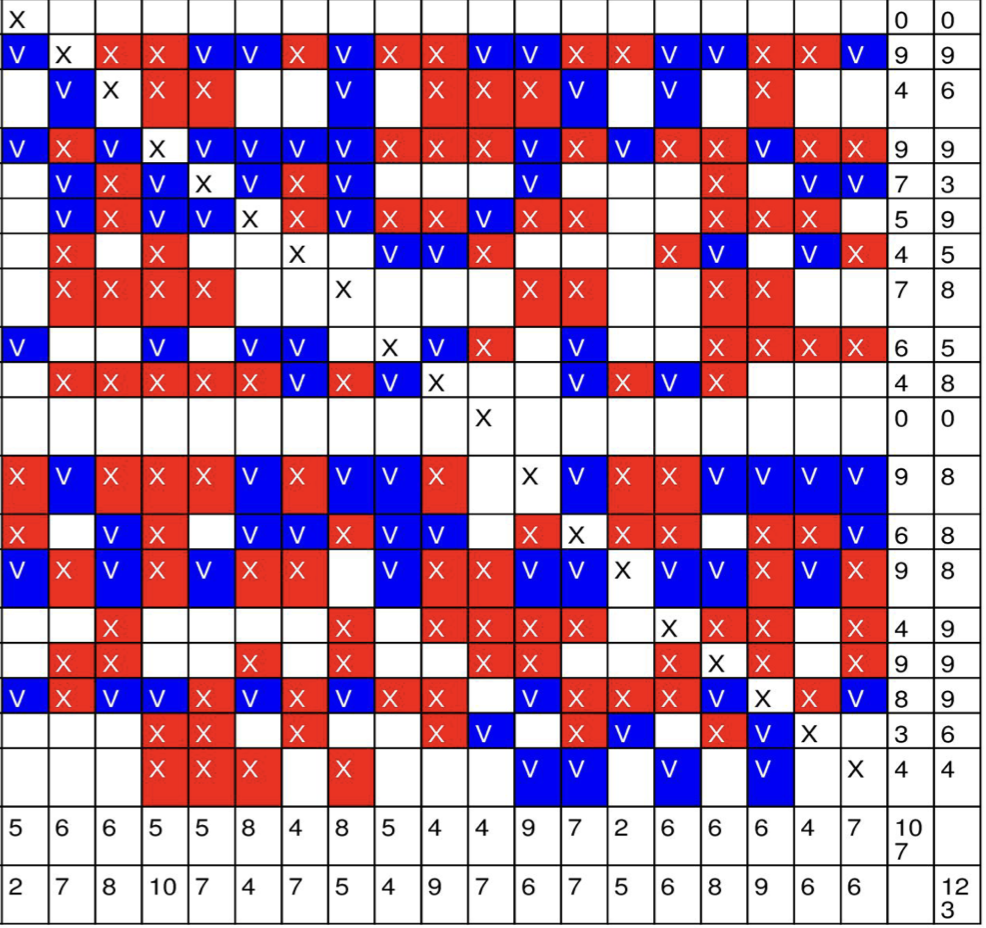
\includegraphics[width=0.4\linewidth]{peers/classe_a} 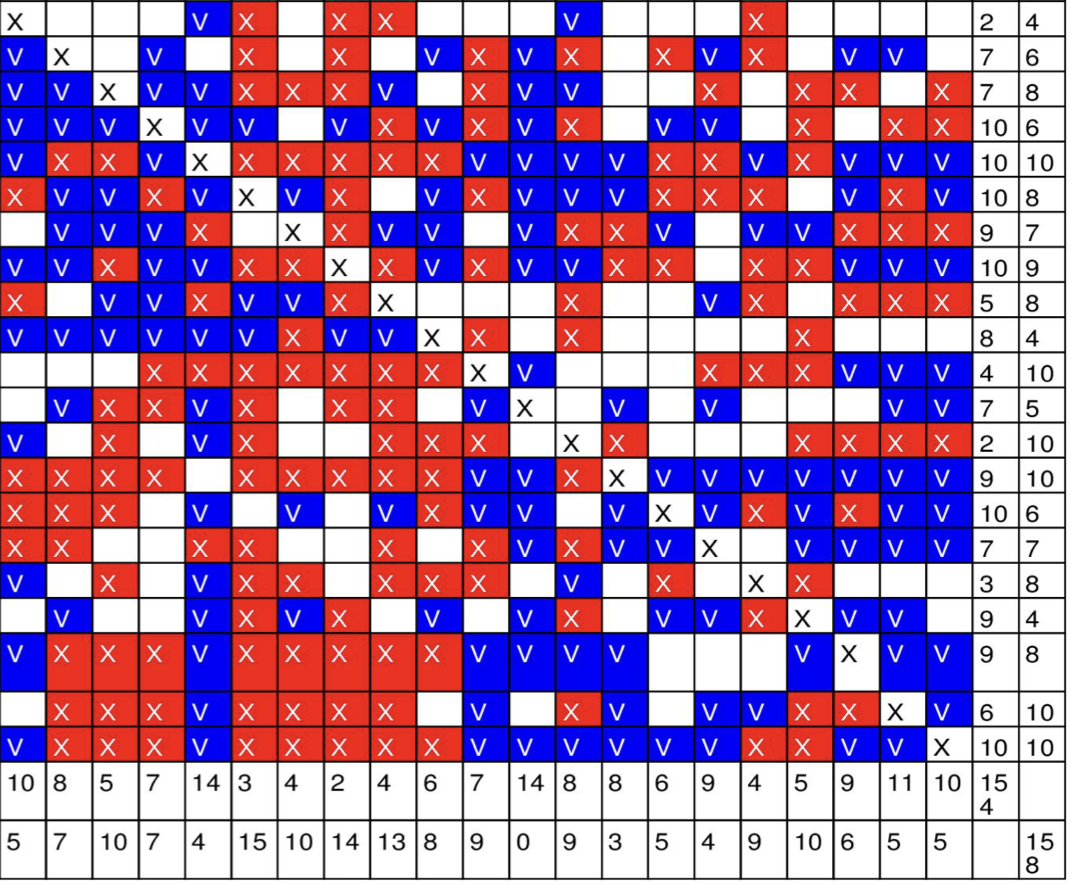
\includegraphics[width=0.4\linewidth]{peers/classe_b} 

}

\caption{Exemples de sociogrammes (extraits anonymisés)}\label{fig:socio}
\end{figure}

\hypertarget{echelle-sep-en-gestion-de-classe}{%
\subsection{Echelle SEP en gestion de classe}\label{echelle-sep-en-gestion-de-classe}}

Le tableau \ref{tab:teach} résume les scores à chacune des 4 dimensions de la gestion de classe (gestion proactive, gestion réactive, implication des parents, implication de personnes externes). Chaque score s'entend sur un maximum de 8.

\begin{verbatim}
## Warning: Warning: fonts used in `flextable` are ignored because the `pdflatex`
## engine is used and not `xelatex` or `lualatex`. You can avoid this warning
## by using the `set_flextable_defaults(fonts_ignore=TRUE)` command or use a
## compatible engine by defining `latex_engine: xelatex` in the YAML header of the
## R Markdown document.
\end{verbatim}

\providecommand{\docline}[3]{\noalign{\global\setlength{\arrayrulewidth}{#1}}\arrayrulecolor[HTML]{#2}\cline{#3}}

\setlength{\tabcolsep}{8pt}

\renewcommand*{\arraystretch}{1.5}

\begin{table}

\centering

\begin{longtable}{|p{0.75in}|p{0.75in}|p{0.75in}|p{0.75in}|p{0.75in}|p{0.75in}}

\caption{Résumé des données pour les 3 enseignantes}\label{tab:teach}\\

\hhline{>{\arrayrulecolor[HTML]{000000}\global\arrayrulewidth=2pt}->{\arrayrulecolor[HTML]{000000}\global\arrayrulewidth=2pt}->{\arrayrulecolor[HTML]{000000}\global\arrayrulewidth=2pt}->{\arrayrulecolor[HTML]{000000}\global\arrayrulewidth=2pt}->{\arrayrulecolor[HTML]{000000}\global\arrayrulewidth=2pt}->{\arrayrulecolor[HTML]{000000}\global\arrayrulewidth=2pt}-}

\multicolumn{1}{!{\color[HTML]{000000}\vrule width 0pt}>{\raggedright}p{\dimexpr 0.75in+0\tabcolsep+0\arrayrulewidth}}{\fontsize{11}{13}\selectfont{\textcolor[HTML]{000000}{Classe}}} & \multicolumn{1}{!{\color[HTML]{000000}\vrule width 0pt}>{\raggedleft}p{\dimexpr 0.75in+0\tabcolsep+0\arrayrulewidth}}{\fontsize{11}{13}\selectfont{\textcolor[HTML]{000000}{Gestion proactive}}} & \multicolumn{1}{!{\color[HTML]{000000}\vrule width 0pt}>{\raggedleft}p{\dimexpr 0.75in+0\tabcolsep+0\arrayrulewidth}}{\fontsize{11}{13}\selectfont{\textcolor[HTML]{000000}{Gestion réactive}}} & \multicolumn{1}{!{\color[HTML]{000000}\vrule width 0pt}>{\raggedleft}p{\dimexpr 0.75in+0\tabcolsep+0\arrayrulewidth}}{\fontsize{11}{13}\selectfont{\textcolor[HTML]{000000}{Impl. des parents}}} & \multicolumn{1}{!{\color[HTML]{000000}\vrule width 0pt}>{\raggedleft}p{\dimexpr 0.75in+0\tabcolsep+0\arrayrulewidth}}{\fontsize{11}{13}\selectfont{\textcolor[HTML]{000000}{Impl. externe}}} & \multicolumn{1}{!{\color[HTML]{000000}\vrule width 0pt}>{\raggedleft}p{\dimexpr 0.75in+0\tabcolsep+0\arrayrulewidth}!{\color[HTML]{000000}\vrule width 0pt}}{\fontsize{11}{13}\selectfont{\textcolor[HTML]{000000}{Total}}} \\

\noalign{\global\setlength{\arrayrulewidth}{2pt}}\arrayrulecolor[HTML]{000000}\cline{1-6}

\endfirsthead

\hhline{>{\arrayrulecolor[HTML]{000000}\global\arrayrulewidth=2pt}->{\arrayrulecolor[HTML]{000000}\global\arrayrulewidth=2pt}->{\arrayrulecolor[HTML]{000000}\global\arrayrulewidth=2pt}->{\arrayrulecolor[HTML]{000000}\global\arrayrulewidth=2pt}->{\arrayrulecolor[HTML]{000000}\global\arrayrulewidth=2pt}->{\arrayrulecolor[HTML]{000000}\global\arrayrulewidth=2pt}-}

\multicolumn{1}{!{\color[HTML]{000000}\vrule width 0pt}>{\raggedright}p{\dimexpr 0.75in+0\tabcolsep+0\arrayrulewidth}}{\fontsize{11}{13}\selectfont{\textcolor[HTML]{000000}{Classe}}} & \multicolumn{1}{!{\color[HTML]{000000}\vrule width 0pt}>{\raggedleft}p{\dimexpr 0.75in+0\tabcolsep+0\arrayrulewidth}}{\fontsize{11}{13}\selectfont{\textcolor[HTML]{000000}{Gestion proactive}}} & \multicolumn{1}{!{\color[HTML]{000000}\vrule width 0pt}>{\raggedleft}p{\dimexpr 0.75in+0\tabcolsep+0\arrayrulewidth}}{\fontsize{11}{13}\selectfont{\textcolor[HTML]{000000}{Gestion réactive}}} & \multicolumn{1}{!{\color[HTML]{000000}\vrule width 0pt}>{\raggedleft}p{\dimexpr 0.75in+0\tabcolsep+0\arrayrulewidth}}{\fontsize{11}{13}\selectfont{\textcolor[HTML]{000000}{Impl. des parents}}} & \multicolumn{1}{!{\color[HTML]{000000}\vrule width 0pt}>{\raggedleft}p{\dimexpr 0.75in+0\tabcolsep+0\arrayrulewidth}}{\fontsize{11}{13}\selectfont{\textcolor[HTML]{000000}{Impl. externe}}} & \multicolumn{1}{!{\color[HTML]{000000}\vrule width 0pt}>{\raggedleft}p{\dimexpr 0.75in+0\tabcolsep+0\arrayrulewidth}!{\color[HTML]{000000}\vrule width 0pt}}{\fontsize{11}{13}\selectfont{\textcolor[HTML]{000000}{Total}}} \\

\noalign{\global\setlength{\arrayrulewidth}{2pt}}\arrayrulecolor[HTML]{000000}\cline{1-6}\endhead



\multicolumn{1}{!{\color[HTML]{000000}\vrule width 0pt}>{\raggedright}p{\dimexpr 0.75in+0\tabcolsep+0\arrayrulewidth}}{\fontsize{11}{13}\selectfont{\textcolor[HTML]{000000}{a}}} & \multicolumn{1}{!{\color[HTML]{000000}\vrule width 0pt}>{\raggedleft}p{\dimexpr 0.75in+0\tabcolsep+0\arrayrulewidth}}{\fontsize{11}{13}\selectfont{\textcolor[HTML]{000000}{4.8}}} & \multicolumn{1}{!{\color[HTML]{000000}\vrule width 0pt}>{\raggedleft}p{\dimexpr 0.75in+0\tabcolsep+0\arrayrulewidth}}{\fontsize{11}{13}\selectfont{\textcolor[HTML]{000000}{6.4}}} & \multicolumn{1}{!{\color[HTML]{000000}\vrule width 0pt}>{\raggedleft}p{\dimexpr 0.75in+0\tabcolsep+0\arrayrulewidth}}{\fontsize{11}{13}\selectfont{\textcolor[HTML]{000000}{3.0}}} & \multicolumn{1}{!{\color[HTML]{000000}\vrule width 0pt}>{\raggedleft}p{\dimexpr 0.75in+0\tabcolsep+0\arrayrulewidth}}{\fontsize{11}{13}\selectfont{\textcolor[HTML]{000000}{5.7}}} & \multicolumn{1}{!{\color[HTML]{000000}\vrule width 0pt}>{\raggedleft}p{\dimexpr 0.75in+0\tabcolsep+0\arrayrulewidth}!{\color[HTML]{000000}\vrule width 0pt}}{\fontsize{11}{13}\selectfont{\textcolor[HTML]{000000}{5.2}}} \\





\multicolumn{1}{!{\color[HTML]{000000}\vrule width 0pt}>{\raggedright}p{\dimexpr 0.75in+0\tabcolsep+0\arrayrulewidth}}{\fontsize{11}{13}\selectfont{\textcolor[HTML]{000000}{a}}} & \multicolumn{1}{!{\color[HTML]{000000}\vrule width 0pt}>{\raggedleft}p{\dimexpr 0.75in+0\tabcolsep+0\arrayrulewidth}}{\fontsize{11}{13}\selectfont{\textcolor[HTML]{000000}{6.0}}} & \multicolumn{1}{!{\color[HTML]{000000}\vrule width 0pt}>{\raggedleft}p{\dimexpr 0.75in+0\tabcolsep+0\arrayrulewidth}}{\fontsize{11}{13}\selectfont{\textcolor[HTML]{000000}{6.8}}} & \multicolumn{1}{!{\color[HTML]{000000}\vrule width 0pt}>{\raggedleft}p{\dimexpr 0.75in+0\tabcolsep+0\arrayrulewidth}}{\fontsize{11}{13}\selectfont{\textcolor[HTML]{000000}{7.0}}} & \multicolumn{1}{!{\color[HTML]{000000}\vrule width 0pt}>{\raggedleft}p{\dimexpr 0.75in+0\tabcolsep+0\arrayrulewidth}}{\fontsize{11}{13}\selectfont{\textcolor[HTML]{000000}{5.7}}} & \multicolumn{1}{!{\color[HTML]{000000}\vrule width 0pt}>{\raggedleft}p{\dimexpr 0.75in+0\tabcolsep+0\arrayrulewidth}!{\color[HTML]{000000}\vrule width 0pt}}{\fontsize{11}{13}\selectfont{\textcolor[HTML]{000000}{6.3}}} \\





\multicolumn{1}{!{\color[HTML]{000000}\vrule width 0pt}>{\raggedright}p{\dimexpr 0.75in+0\tabcolsep+0\arrayrulewidth}}{\fontsize{11}{13}\selectfont{\textcolor[HTML]{000000}{b}}} & \multicolumn{1}{!{\color[HTML]{000000}\vrule width 0pt}>{\raggedleft}p{\dimexpr 0.75in+0\tabcolsep+0\arrayrulewidth}}{\fontsize{11}{13}\selectfont{\textcolor[HTML]{000000}{6.8}}} & \multicolumn{1}{!{\color[HTML]{000000}\vrule width 0pt}>{\raggedleft}p{\dimexpr 0.75in+0\tabcolsep+0\arrayrulewidth}}{\fontsize{11}{13}\selectfont{\textcolor[HTML]{000000}{7.2}}} & \multicolumn{1}{!{\color[HTML]{000000}\vrule width 0pt}>{\raggedleft}p{\dimexpr 0.75in+0\tabcolsep+0\arrayrulewidth}}{\fontsize{11}{13}\selectfont{\textcolor[HTML]{000000}{7.5}}} & \multicolumn{1}{!{\color[HTML]{000000}\vrule width 0pt}>{\raggedleft}p{\dimexpr 0.75in+0\tabcolsep+0\arrayrulewidth}}{\fontsize{11}{13}\selectfont{\textcolor[HTML]{000000}{7.7}}} & \multicolumn{1}{!{\color[HTML]{000000}\vrule width 0pt}>{\raggedleft}p{\dimexpr 0.75in+0\tabcolsep+0\arrayrulewidth}!{\color[HTML]{000000}\vrule width 0pt}}{\fontsize{11}{13}\selectfont{\textcolor[HTML]{000000}{7.2}}} \\

\noalign{\global\setlength{\arrayrulewidth}{2pt}}\arrayrulecolor[HTML]{000000}\cline{1-6}

\end{longtable}

\end{table}

\hypertarget{echelle-bien-uxeatre-uxe0-luxe9cole}{%
\subsection{Echelle Bien-être à l'école}\label{echelle-bien-uxeatre-uxe0-luxe9cole}}

Le tableau \ref{tab:peers} indique le niveau de bien-être par classe (le score maximal vaut 7).

\begin{verbatim}
## Warning: Warning: fonts used in `flextable` are ignored because the `pdflatex`
## engine is used and not `xelatex` or `lualatex`. You can avoid this warning
## by using the `set_flextable_defaults(fonts_ignore=TRUE)` command or use a
## compatible engine by defining `latex_engine: xelatex` in the YAML header of the
## R Markdown document.
\end{verbatim}

\providecommand{\docline}[3]{\noalign{\global\setlength{\arrayrulewidth}{#1}}\arrayrulecolor[HTML]{#2}\cline{#3}}

\setlength{\tabcolsep}{8pt}

\renewcommand*{\arraystretch}{1.5}

\begin{table}

\centering

\begin{longtable}{|p{0.75in}|p{0.75in}|p{0.75in}|p{0.75in}|p{0.75in}|p{0.75in}}

\caption{Résumé des scores de bien-être pour les 2 classes}\label{tab:peers}\\

\hhline{>{\arrayrulecolor[HTML]{000000}\global\arrayrulewidth=2pt}->{\arrayrulecolor[HTML]{000000}\global\arrayrulewidth=2pt}->{\arrayrulecolor[HTML]{000000}\global\arrayrulewidth=2pt}->{\arrayrulecolor[HTML]{000000}\global\arrayrulewidth=2pt}->{\arrayrulecolor[HTML]{000000}\global\arrayrulewidth=2pt}->{\arrayrulecolor[HTML]{000000}\global\arrayrulewidth=2pt}-}

\multicolumn{1}{!{\color[HTML]{000000}\vrule width 0pt}>{\raggedright}p{\dimexpr 0.75in+0\tabcolsep+0\arrayrulewidth}}{\fontsize{11}{13}\selectfont{\textcolor[HTML]{000000}{Classe}}} & \multicolumn{1}{!{\color[HTML]{000000}\vrule width 0pt}>{\raggedleft}p{\dimexpr 0.75in+0\tabcolsep+0\arrayrulewidth}}{\fontsize{11}{13}\selectfont{\textcolor[HTML]{000000}{Moyenne}}} & \multicolumn{1}{!{\color[HTML]{000000}\vrule width 0pt}>{\raggedleft}p{\dimexpr 0.75in+0\tabcolsep+0\arrayrulewidth}}{\fontsize{11}{13}\selectfont{\textcolor[HTML]{000000}{Score maxium}}} & \multicolumn{1}{!{\color[HTML]{000000}\vrule width 0pt}>{\raggedleft}p{\dimexpr 0.75in+0\tabcolsep+0\arrayrulewidth}}{\fontsize{11}{13}\selectfont{\textcolor[HTML]{000000}{Score minimum}}} & \multicolumn{1}{!{\color[HTML]{000000}\vrule width 0pt}>{\raggedleft}p{\dimexpr 0.75in+0\tabcolsep+0\arrayrulewidth}}{\fontsize{11}{13}\selectfont{\textcolor[HTML]{000000}{Médiane}}} & \multicolumn{1}{!{\color[HTML]{000000}\vrule width 0pt}>{\raggedleft}p{\dimexpr 0.75in+0\tabcolsep+0\arrayrulewidth}!{\color[HTML]{000000}\vrule width 0pt}}{\fontsize{11}{13}\selectfont{\textcolor[HTML]{000000}{Ecart-type}}} \\

\noalign{\global\setlength{\arrayrulewidth}{2pt}}\arrayrulecolor[HTML]{000000}\cline{1-6}

\endfirsthead

\hhline{>{\arrayrulecolor[HTML]{000000}\global\arrayrulewidth=2pt}->{\arrayrulecolor[HTML]{000000}\global\arrayrulewidth=2pt}->{\arrayrulecolor[HTML]{000000}\global\arrayrulewidth=2pt}->{\arrayrulecolor[HTML]{000000}\global\arrayrulewidth=2pt}->{\arrayrulecolor[HTML]{000000}\global\arrayrulewidth=2pt}->{\arrayrulecolor[HTML]{000000}\global\arrayrulewidth=2pt}-}

\multicolumn{1}{!{\color[HTML]{000000}\vrule width 0pt}>{\raggedright}p{\dimexpr 0.75in+0\tabcolsep+0\arrayrulewidth}}{\fontsize{11}{13}\selectfont{\textcolor[HTML]{000000}{Classe}}} & \multicolumn{1}{!{\color[HTML]{000000}\vrule width 0pt}>{\raggedleft}p{\dimexpr 0.75in+0\tabcolsep+0\arrayrulewidth}}{\fontsize{11}{13}\selectfont{\textcolor[HTML]{000000}{Moyenne}}} & \multicolumn{1}{!{\color[HTML]{000000}\vrule width 0pt}>{\raggedleft}p{\dimexpr 0.75in+0\tabcolsep+0\arrayrulewidth}}{\fontsize{11}{13}\selectfont{\textcolor[HTML]{000000}{Score maxium}}} & \multicolumn{1}{!{\color[HTML]{000000}\vrule width 0pt}>{\raggedleft}p{\dimexpr 0.75in+0\tabcolsep+0\arrayrulewidth}}{\fontsize{11}{13}\selectfont{\textcolor[HTML]{000000}{Score minimum}}} & \multicolumn{1}{!{\color[HTML]{000000}\vrule width 0pt}>{\raggedleft}p{\dimexpr 0.75in+0\tabcolsep+0\arrayrulewidth}}{\fontsize{11}{13}\selectfont{\textcolor[HTML]{000000}{Médiane}}} & \multicolumn{1}{!{\color[HTML]{000000}\vrule width 0pt}>{\raggedleft}p{\dimexpr 0.75in+0\tabcolsep+0\arrayrulewidth}!{\color[HTML]{000000}\vrule width 0pt}}{\fontsize{11}{13}\selectfont{\textcolor[HTML]{000000}{Ecart-type}}} \\

\noalign{\global\setlength{\arrayrulewidth}{2pt}}\arrayrulecolor[HTML]{000000}\cline{1-6}\endhead



\multicolumn{1}{!{\color[HTML]{000000}\vrule width 0pt}>{\raggedright}p{\dimexpr 0.75in+0\tabcolsep+0\arrayrulewidth}}{\fontsize{11}{13}\selectfont{\textcolor[HTML]{000000}{a}}} & \multicolumn{1}{!{\color[HTML]{000000}\vrule width 0pt}>{\raggedleft}p{\dimexpr 0.75in+0\tabcolsep+0\arrayrulewidth}}{\fontsize{11}{13}\selectfont{\textcolor[HTML]{000000}{6}}} & \multicolumn{1}{!{\color[HTML]{000000}\vrule width 0pt}>{\raggedleft}p{\dimexpr 0.75in+0\tabcolsep+0\arrayrulewidth}}{\fontsize{11}{13}\selectfont{\textcolor[HTML]{000000}{7}}} & \multicolumn{1}{!{\color[HTML]{000000}\vrule width 0pt}>{\raggedleft}p{\dimexpr 0.75in+0\tabcolsep+0\arrayrulewidth}}{\fontsize{11}{13}\selectfont{\textcolor[HTML]{000000}{1.8}}} & \multicolumn{1}{!{\color[HTML]{000000}\vrule width 0pt}>{\raggedleft}p{\dimexpr 0.75in+0\tabcolsep+0\arrayrulewidth}}{\fontsize{11}{13}\selectfont{\textcolor[HTML]{000000}{6.6}}} & \multicolumn{1}{!{\color[HTML]{000000}\vrule width 0pt}>{\raggedleft}p{\dimexpr 0.75in+0\tabcolsep+0\arrayrulewidth}!{\color[HTML]{000000}\vrule width 0pt}}{\fontsize{11}{13}\selectfont{\textcolor[HTML]{000000}{1.37}}} \\





\multicolumn{1}{!{\color[HTML]{000000}\vrule width 0pt}>{\raggedright}p{\dimexpr 0.75in+0\tabcolsep+0\arrayrulewidth}}{\fontsize{11}{13}\selectfont{\textcolor[HTML]{000000}{b}}} & \multicolumn{1}{!{\color[HTML]{000000}\vrule width 0pt}>{\raggedleft}p{\dimexpr 0.75in+0\tabcolsep+0\arrayrulewidth}}{\fontsize{11}{13}\selectfont{\textcolor[HTML]{000000}{6}}} & \multicolumn{1}{!{\color[HTML]{000000}\vrule width 0pt}>{\raggedleft}p{\dimexpr 0.75in+0\tabcolsep+0\arrayrulewidth}}{\fontsize{11}{13}\selectfont{\textcolor[HTML]{000000}{7}}} & \multicolumn{1}{!{\color[HTML]{000000}\vrule width 0pt}>{\raggedleft}p{\dimexpr 0.75in+0\tabcolsep+0\arrayrulewidth}}{\fontsize{11}{13}\selectfont{\textcolor[HTML]{000000}{3.8}}} & \multicolumn{1}{!{\color[HTML]{000000}\vrule width 0pt}>{\raggedleft}p{\dimexpr 0.75in+0\tabcolsep+0\arrayrulewidth}}{\fontsize{11}{13}\selectfont{\textcolor[HTML]{000000}{6.2}}} & \multicolumn{1}{!{\color[HTML]{000000}\vrule width 0pt}>{\raggedleft}p{\dimexpr 0.75in+0\tabcolsep+0\arrayrulewidth}!{\color[HTML]{000000}\vrule width 0pt}}{\fontsize{11}{13}\selectfont{\textcolor[HTML]{000000}{0.92}}} \\

\noalign{\global\setlength{\arrayrulewidth}{2pt}}\arrayrulecolor[HTML]{000000}\cline{1-6}

\end{longtable}

\end{table}

La représentation graphique \ref{fig:vis} nous donne une idée de la distribution des scores, par classe.

\begin{figure}

{\centering 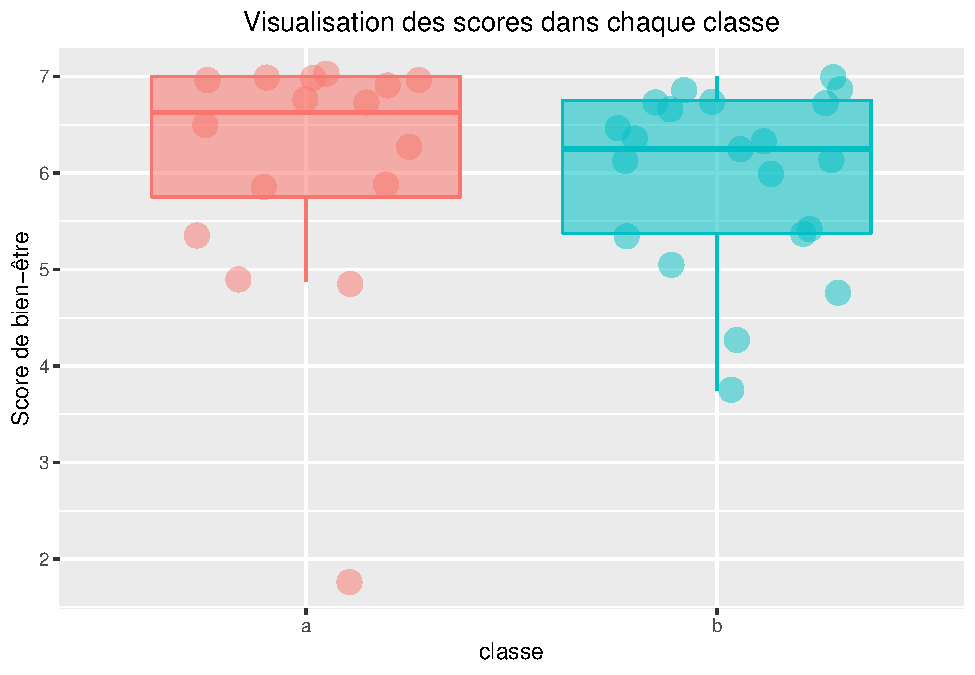
\includegraphics[width=0.8\linewidth]{hlm2020_nb_rapport_files/figure-latex/vis-1} 

}

\caption{distribution des scores}\label{fig:vis}
\end{figure}

\hypertarget{echelle-de-ruxe9gulation-uxe9motionnelle}{%
\subsection{Echelle de Régulation émotionnelle}\label{echelle-de-ruxe9gulation-uxe9motionnelle}}

\emph{Données en main des personnes-ressources (identification des éventuels besoins)}

\hypertarget{echelle-de-compuxe9tences-psychosociales}{%
\subsection{Echelle de compétences psychosociales}\label{echelle-de-compuxe9tences-psychosociales}}

\emph{Données en main des personnes-ressources (identification des éventuels besoins)}

\end{document}
